%!TEX root = ../report.tex

\begin{document}
    \chapter{Introduction}
    In recent years the development of deep learning and improvement in hardware has led rapidly to the advancement of autonomous driving technology. Traditionally modular methods were used for self-driving systems. In a modular self-driving software stack we have independent modules like perception, path-planning, localization, and control which are generally interconnected to each other. The main advantage of modular methods is that they are interpretable in case of any faulty modules but maintaining and developing such modules is costly and time-consuming. Moreover, modular-based stacks are still far from complete autonomy for autonomous driving.
    \par Nowadays research in autonomous driving is shifted towards end-to-end-based approaches. In end-to-end autonomous driving, all the sensory inputs are fed into a single neural network architecture, which is responsible for lateral and longitudinal control of the car.  An end-to-end driving pipeline is generally simpler than a modular stack, which is trained in a supervised manner using imitation learning techniques \cite{DBLP:journals/corr/abs-1710-02410}, \cite{pan2019agile} where a neural network is trained to mimic expert human driving behavior or sometimes by exploring the environment and learning the driving policy by reinforcement-learning-based techniques. \cite{DBLP:journals/corr/abs-1807-00412}.  

     \begin{figure}[h]
    \centering
    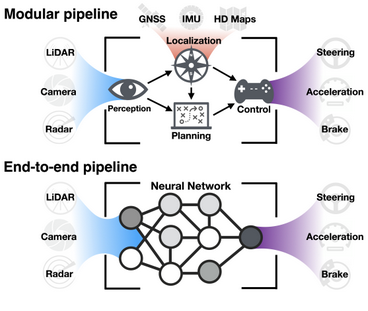
\includegraphics[width=8cm, height=7cm]{images/Modularvsend.png}
    \caption{Comparison between modular and end-to-end approaches for autonomous driving \cite{DBLP:journals/corr/abs-2003-06404}}
    \end{figure}
    
    \section{Motivation an Challenges}
    According to a top market research firm \cite{market_survey}, the autonomous car market size is worth 1.45 billion USD in 2020, and irrespective of the global impact of Covid-19 it is projected to grow to 11.03 billion USD in 2028. A large part of this allurement towards this sector is because of the advancement in sensor technology and new technologies in the field of self-driving. Big companies like Tesla, Lyft, Uber, and CommaAI are fighting to release the first full self-driving software stack. 
\par The simplicity of end-to-end self driving comes at cost of interpret-ability of the results, where a deep neural network is treated as a black-box when there are no intermediate outputs and it is impossible to judge the uncertainty in the predictions from the neural network. To solve the main drawback of the end-to-end-based approaches researchers opt to go for techniques where they take help of some intermediate tasks called auxiliary tasks. These auxiliary tasks in general capture aspects of a scene like lead car position, dynamic objects, traffic signs, behavior of pedestrians, road markings thus quantifying the decisions of the trained driving policy. 

 \begin{figure}[h]
    \centering
    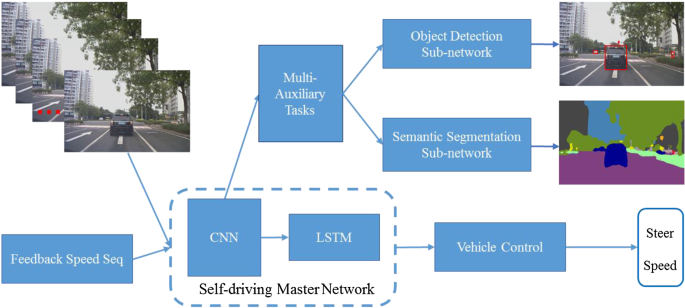
\includegraphics[width=12cm, height=6cm]{images/replace1.png}
    \caption{End-to-end autonomous driving with auxiliary tasks \cite{Wang2019EndtoEndSU}}
\end{figure}

\par In general these auxiliary tasks share the same intermediate layers in the network and any failure in the auxiliary task will indicate the presence of incomplete information in the scene. These tasks are optimized simultaneously using multiple loss functions or a combined weighted loss function according to the importance of the task. Optimizing such auxiliary tasks along with the main task helps the network to learn better the internal representations of the scene as some tasks share some meaningful information. Thus such approaches to learning auxiliary tasks along with the main driving task can be categorized as  multi-task learning problems. Multi-task learning has provided concrete results on applications of machine learning like natural language processing \cite{nlp}, computer vision \cite{DBLP:journals/corr/abs-2002-05347}, speech recognition \cite{qiu2021multitask}.    
End-to-end autonomous driving via imitation learning, in general suffers from other challenges like: 

\begin{itemize}
\item Causal confusion - imitation learning datasets contain more common scenarios like driving straight, thus  generally are not balanced. The inputs to the model are high dimensional and any correlations can result in causal confusion. 
\item Distribution Shift - an imitation learning model imitates expert's driving behaviour. Inferring the trained model in real world can lead to scenarios unseen during training and model will not be able to respond appropriately to such scenarios. 
\item Task Loss balancing - define a suitable task loss balancing strategy for the multi-task network for efficient learning.
\item Simulation can not cover all the scenarios.
\item Selection of a unified feature extractor for the multi-task end-to-end network.
\item Selection of auxiliary tasks for the prediction of appropriate driving commands. 
\end{itemize}

    \section{Problem Statement}
    This project aims at predicting road lanes in 3D and driving commands using a single or sequence of monocular images in an end-to-end manner. The whole task in general can be treated as a multitask learning problem where 3d lane detection is obtained as an auxiliary task. The project further aims to investigate the following.
    
    \begin{itemize}
 \item Efficacy of using 3d lane detection as an auxiliary task to enhance the performance of the main task that is driving commands.
\item Interpretability of the pipeline by introducing auxiliary tasks. 
\item Can multitask learning improve generalization? 
\item Can task loss balancing favor the performance of the main task?  
\end{itemize}

3D lane detection pipeline will be trained and evaluated on a synthetic Apollo 3D \cite{guo2020gen} dataset. Whereas, training for driving commands can be carried out via any large scale autonomous driving dataset which contain video data and vehicle canbus information like Comma2k19 \cite{1812.05752},  Cityscapes \cite{DBLP:journals/corr/CordtsORREBFRS16}, Nuscenes \cite{DBLP:journals/corr/abs-1903-11027}.
\end{document}
